\newpage
\section{Branch-and-Bound Technique for Solving Integer Programs}

% Principi dell'algoritmo Branch-and-Bound
\subsection{Principi dell'argoritmo Branch-and-Bound}

I problemi che cerchiamo di risolvere sono \hl{lineari con variabli decisionali}, il problema è che \hl{alcune variabili possono essere intere}, o anche binarie, al posto di essere continue. Per questi casi abbiamo alcuni \hl{approcci naive} da usare:

\begin{enumerate}
    \item \hl{brute force}: se abbiamo n variabili binarie le soluzioni ammissibili sono $2^n$. Andremo quindi a \textbf{generare tutte le soluzioni e verficarne i vincoli} sono soddisfatti (non computazionalmente possibile)
    \item \hl{rounding}: sostituisco le variabili intere con un "rilassamento" del vincolo di integrità. Quindi il problema \textbf{$P$}:
        $$\max z = 3x_1 + 4x_2 - 2x_3 + 3x_4 - 2x_5$$

        con vincoli:
        \begin{itemize}
            \item $2x_1 + 2x_2 + 2x_3 + 2x_4 + 2x_5 \leq 4$
            \item $x_1, x_2, x_3, x_4, x_5 = 0/1$
        \end{itemize}

        diventa \textbf{$R(P)$}:
        $$\max z = 3x_1 + 4x_2 – 2x_3 + 3x_4 – 2x_5$$
        
        con vincoli:
        \begin{itemize}
            \item $2x_1 + 2x_2 + 2x_3 + 2x_4 + 2x_5 \leq 4$
            \item $0 \leq x_1, x_2, x_3, x_4, x_5 \leq 1$
        \end{itemize}
        
        Avremo un \textbf{caso fortunato} se la soluzione di $R(P)$ è anche quella di $P$.

\end{enumerate}


% Approccio Branch-and-Bound
\subsection{Approccio Branch-and-Bound}

È detta tecnica di enumeramerazione parsiale dove \hl{ci si procura una stima del valore della soluzione ottima rilassando il vincolo di integrita'} sulle veriabili intere.

Nella sua risoluzione tramite blackbox potremo avere \hl{4 casistiche}:

\begin{enumerate}
    \item \hl{$R(P)$ inammissibile} $\to$ $P$ inammissibile:
    
        \begin{figure}[H]
        \centering
        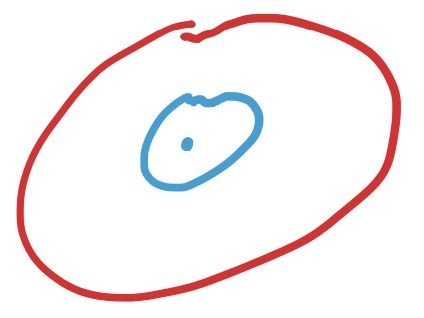
\includegraphics[scale=0.2]{rpp.jpeg}
        \caption{$R(P)$ che contiene $P$} 
        \label{rpp}
        \end{figure}
    
    \item $R(P)$ unbounded $\to$ \hl{$P$ puo' essere unbounded} (dove abbiamo variabili intere):
    
        \begin{figure}[H]
        \centering
        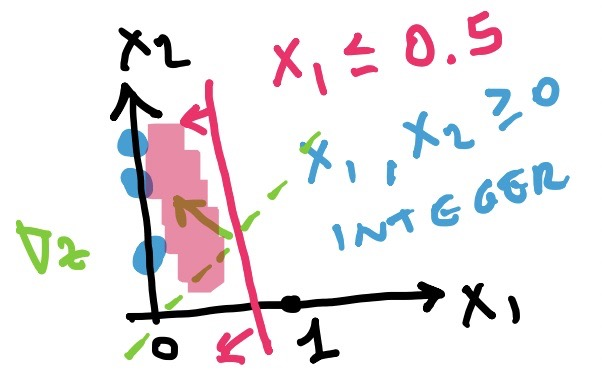
\includegraphics[scale=0.2]{cas1.jpeg}
        \caption{In caso di $P$ unbounded} 
        \label{cas1}
        \end{figure}
    
    \item $R(P)$ unbounded $\to$ \hl{$P$ puo' essere inammissibile} (dove non abbiamo variabili intere):
    
        \begin{figure}[H]
        \centering
        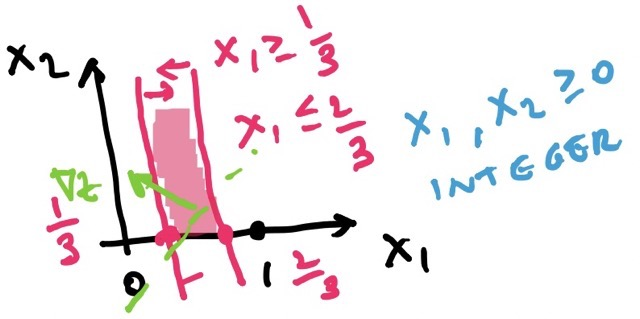
\includegraphics[scale=0.25]{cas2.jpeg}
        \caption{In caso di $P$ inammissibile} 
        \label{cas2}
        \end{figure}

        (p.s: non posso saperlo dato che la blackbox mi sa solo $R(P)$)

    \item \hl{$R(P)$ ha soluzione ottima} $\to$ $P$ inammissibile
        
        \begin{figure}[H]
        \centering
        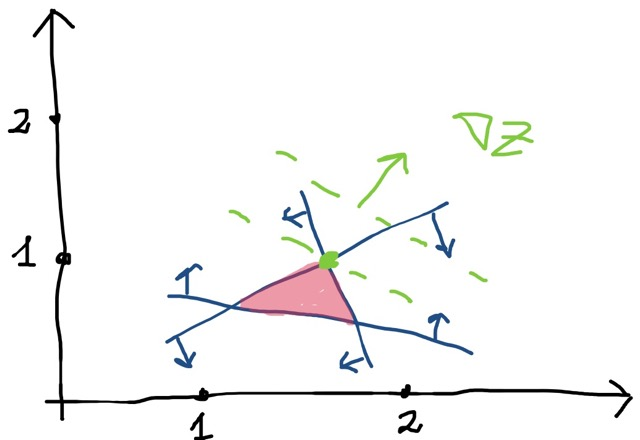
\includegraphics[scale=0.25]{pin.jpeg}
        \caption{$R(P)$ ottima ma $P$ inammissibile} 
        \label{pin}
        \end{figure}

        (p.s: non posso saperlo dato che la blackbox mi sa solo $R(P)$)

    \item \hl{$R(P)$ ha soluzione ottima} $\to$ $P$ ammissibile
        
        \begin{figure}[H]
        \centering
        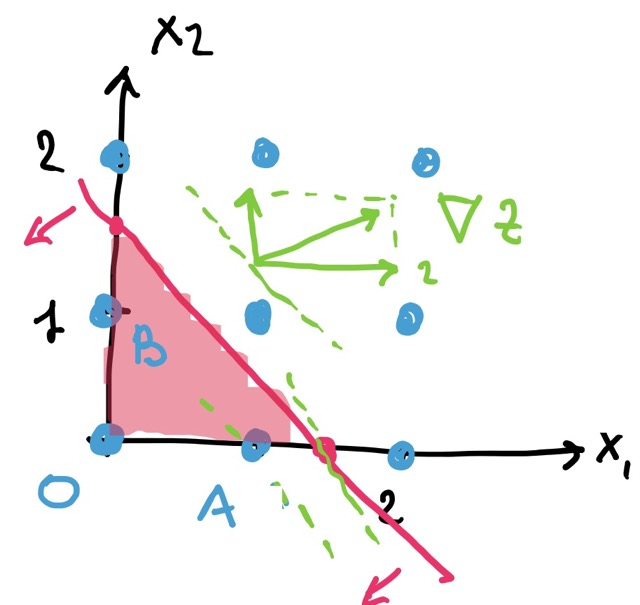
\includegraphics[scale=0.25]{pam.jpeg}
        \caption{$R(P)$ ottima ma $P$ ammissibile} 
        \label{pam}
        \end{figure}

        dove avremo come \textbf{soluzioni intere}:
        $$O(0,0),\ A(1,0),\ B(0, 1)$$

        Andrò allora a \textbf{traslare al curva di livello} fino a trovare la \textbf{soluzione $R(P)$: primo numero ammissibile} nella regione ammissibile, nceve \textbf{per $P$: primo numero intero ammissibile}

\end{enumerate}

La \hl{soluzione ottima di ottimizzazione sara' quella di $R(P)$} di rilassamento continuo, perché \hl{ha meno vincoli} fornendo una soluzione migliore o uguale della nostra stima. Allora se massimizziamo:
$$Z^*_{R(P)} \geq Z^*_P$$

se sto minimizzando:
$$Z^*_{R(P)} \leq Z^*_P$$

dove avrò rispettivamente \hl{upper-bound} e \hl{lower-bound}.


% Branching
\subsection{Branching}

Oltre ad upper-bound e lower-bound su effettua un \hl{branch} cioè una \hl{suddivisione del problema in sottoproblemi}, dove per le soluzioni ammissibili (s.a.):

\begin{itemize}
    \item $P$ s.a. = $P_1$ s.a. $\cup$ $P_2$ s.a.
    \item $P_1$ s.a. $\cap$ $P_2$ s.a. = insieme vuoto
    \item $\underline{x}^*$ $\notin$ $P_1$ s.a., $P_2$ s.a.
\end{itemize}

con $\underline{x}^*$ possibile vincolo applicabile a $x_1$ o $x_2$. Infatti per un problema a 2 variabili abbiamo:

\begin{figure}[H]
\centering
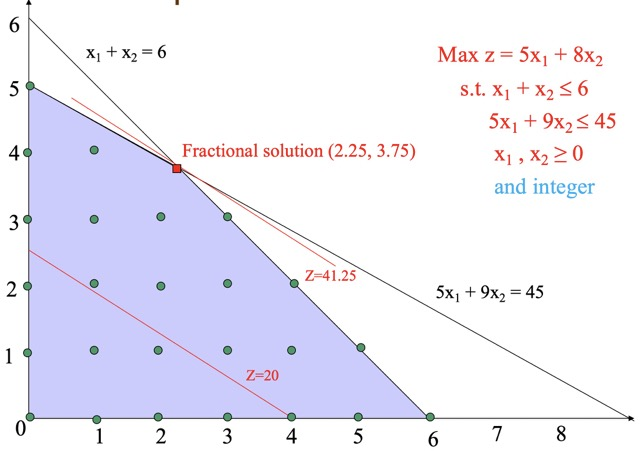
\includegraphics[scale=0.4]{branchprob.jpeg}
\caption{Problema di branching} 
\label{branchprob}
\end{figure}

con soluzione ottima in $(2.25, 3.75)$ con upper: $z = 41.25$.

\hl{Avendo dei valori frazionari effetttuo un branch} per creare dei sottoproblemi. Avendo la soluzione in $(2.25, 3.75)$ allora effettuo il "troncamento" in:
$$x_2 \leq 3,\ x_2 \geq 4$$

\begin{figure}[H]
\centering
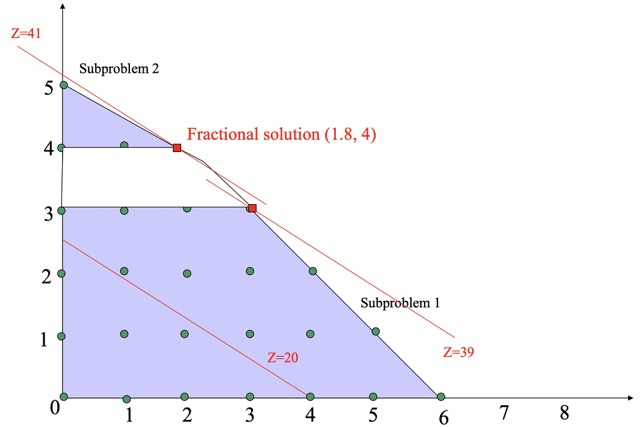
\includegraphics[scale=0.4]{child1.jpeg}
\caption{Primo child} 
\label{child1}
\end{figure}

Quindi per il \hl{sottoproblema $P_1$} con f.o:
$$\max z = 5x_1 + 8x_2$$

e vincoli:
\begin{itemize}
    \item $x_1 + x_2 \leq 6$
    \item $5x_1 + 9x_2 \leq 45$
    \item $x_2 \leq 3$
    \item $x_1,\ x_2 \geq 0$
\end{itemize}

che avrà come \hl{soluzione} $(3, 3)$ con uppeboound $z = 39$.

invece per il \hl{sottoproblema $P_2$} con f.o:
$$\max z = 5x_1 + 8x_2$$

e vincoli:
\begin{itemize}
    \item $x_1 + x_2 \leq 6$
    \item $5x_1 + 9x_2 \leq 45$
    \item $x_2 \geq 4$
    \item $x_1,\ x_2 \geq 0$
\end{itemize}

che avrà come \hl{soluzione} $(1.8, 4)$ con uppeboound $z = 41$.

Avendo \hl{numeri interi in $P_1$} ho una soluzione ottima e non dovrò fare branch su $P_1$ e dato il suo valore di $z$ che è \hl{cerco in $P_2$} con f.o:
risolveremo allora risolvendo il sottoproblema 1 con soluzione 3, 3 con z = 39 allora non ho bisogno di eplorare ancora dato che ho già la soluzione ottima \hl{minore di quello di $P_2$} allora: \hl{scarto $P_1$ e continuo i branch su $P_2$}.


\begin{figure}[H]
\centering
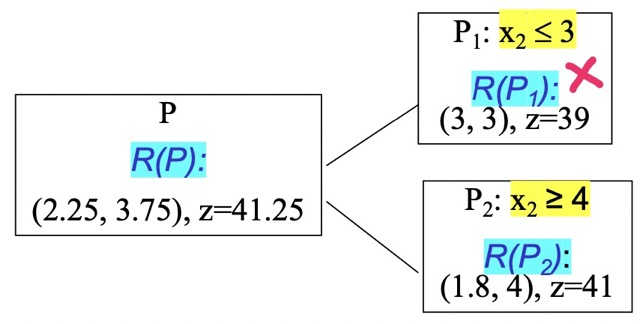
\includegraphics[scale=0.4]{nop1.jpeg}
\caption{Scarto del primo child} 
\label{nop1}
\end{figure}


Effettuando il branch avremo:

\begin{itemize}
    \item \hl{$P_3$}: con vincolo $x_1 \leq 1$
    \item \hl{$P_4$}: con vincolo $x_1 \geq 2$
\end{itemize}

tenendo in conto che \hl{i child ereditano i vincoli del parent}, risolviamo i loro rilassamenti:

\begin{itemize}
    \item \hl{$P_4$}: $R(P_4)$ inammissibile, dato che non ha intersezioni, allora anche P lo sarà
    \item \hl{$P_3$}:$R(P_3)$ avrà $(1, 4.44)$ con $z = 40.55$
\end{itemize}


\begin{figure}[H]
\centering
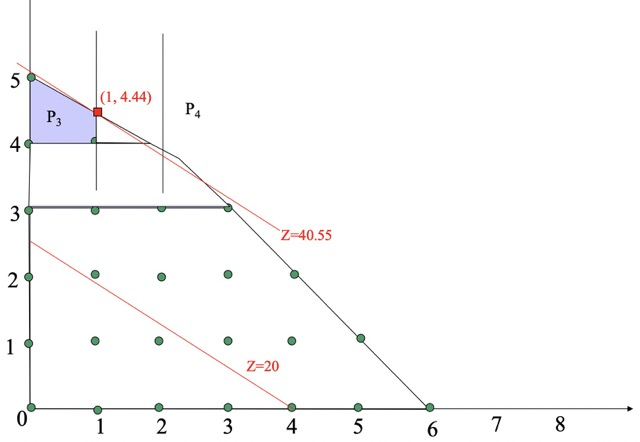
\includegraphics[scale=0.4]{child2.jpeg}
\caption{Secondo child} 
\label{child2}
\end{figure}

\begin{figure}[H]
\centering
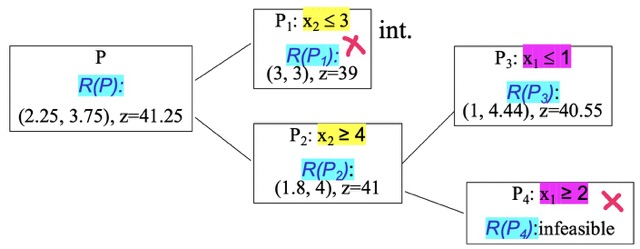
\includegraphics[scale=0.4]{nop4.jpeg}
\caption{Scarto del secondo child} 
\label{nop4}
\end{figure}


continuando con il branch avremo:

\begin{itemize}
    \item \hl{$P_5$}: con $x_2 \leq 4$ con $(1, 4)$ con $z = 37$
    \item \hl{$P_6$}: con $x_2 \geq 5$ con $(0, 5)$ con $z = 40$
\end{itemize} 

scartiamo allora $P_5$ che ci fa arrivare ad un massimo di $37 < 40$ di $P_6$:

\begin{figure}[H]
\centering
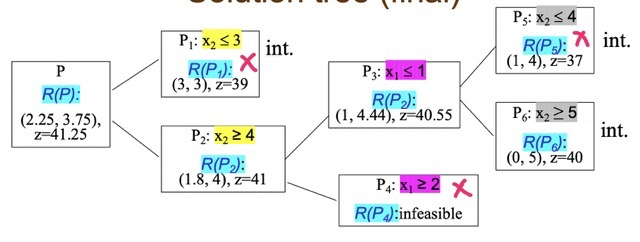
\includegraphics[scale=0.4]{nop56.jpeg}
\caption{Scarto del terzo child} 
\label{nop56}
\end{figure}

\begin{figure}[H]
\centering
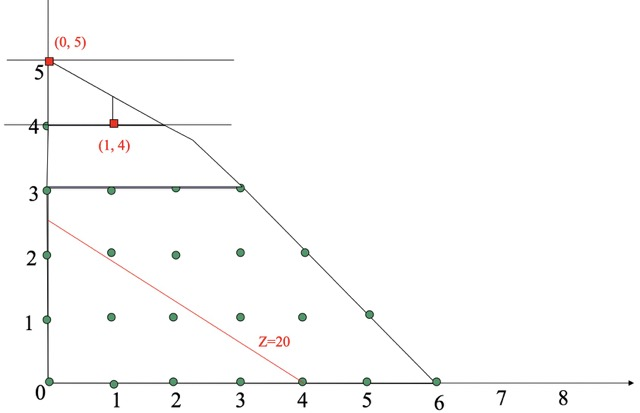
\includegraphics[scale=0.4]{child3.jpeg}
\caption{Terzo child} 
\label{child3}
\end{figure}


siamo quindi arrivati nella situazione in cui \hl{non ci sono piu' branch da creare}.


% Fathoming
\subsection{Fathoming}

Completa l'analisi dei sottoproblemi dicendo che \hl{posso eliminare un sottoproblema} se:

\begin{itemize}
    \item il \hl{rilassamento e' inammissibile}
    \item il rilassamento di $P$ \hl{($R(P)$) ha soluzione ottima intera}, allora è anche soluzione di $P$
    \item è verificato il \hl{fenomeno di dominanza}, quindi una $z$ è più grande delle altre
\end{itemize}

Lo \hl{pseudocodice} è:

\begin{itemize}
    \item[] $L := \{P\}$ // lista dei sottoproblemi da analizzare
    \item[] $z^{\text{best}} := -\infty$
    \item[] $x^{\text{best}} := \text{NULL}$
    \item[] while $L$ è vuoto:
    \begin{itemize}
        \item[] estrarre un sottoproblema $k$ da $L$
        \item[] branching da $1 \to n_k$
        \item[] risolvo $R(P)$ e trovo i limiti e l'upperbound $UB$
        \item[] for $i = 1$ to $n_k$:
        \begin{itemize}
            \item[] if $UB_i \leq z^{\text{best}}$ then:
            \begin{itemize}
                \item[] kill $\text{child}_i$
            \end{itemize}
            \item[] elif $R(P)$ è una soluzione intera:
            \begin{itemize}
                \item[] $z^{\text{best}} := UB_i$
                \item[] $x^{\text{best}} := \text{child}_i$
            \end{itemize}
            \item[] elif $R(P)$ è una soluzione frazionaria:
            \begin{itemize}
                \item[] add $\text{child}_i$ to $L$
            \end{itemize}
        \end{itemize}
        \item[] end for
    \end{itemize}
    \item[] end while
\end{itemize}


% Esercizio Branch-and-Bound
\subsection{Esercizio Branch-and-Bound}

Funzione obiettivo:
$$\max z = x_1 + x_2$$

v.o:

\begin{itemize}
    \item $-6x_1 + 12x_2 \leq 9$
    \item $6x_1 - 4x_2 \leq 9$
    \item $x_1, x_2 \geq 0$
\end{itemize}

gradiente:

$$\nabla z =
\left[ {\begin{array}{c}
	1 \\
	1 \\
\end{array} } \right]
$$

grafico:

\begin{figure}[H]
\centering
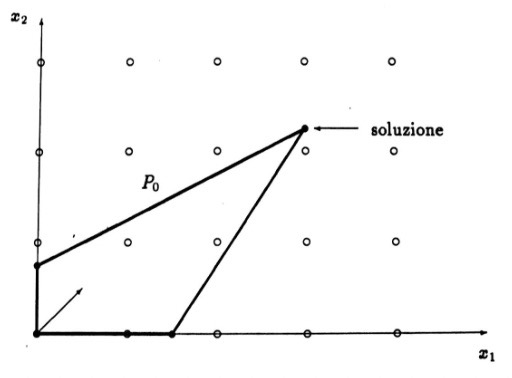
\includegraphics[scale=0.4]{grafbab.jpeg}
\caption{Regione ammissibile} 
\label{grafbab}
\end{figure}

abbiamo che la soluzione ottima (l'intersezione) del risultato continuo è:
$$x_1 = 3,\ x_2 = 2.25,\ z = 5.25$$

allora prenderemo come upper-bound $5$.

La variabile $x_2$ ha valore frazionario compreso tra $2$ e $3$. Effettuiamo un branch con vincoli $x_2 \leq 2$ e $x_2 \geq 3$:

\begin{figure}[H]
\centering
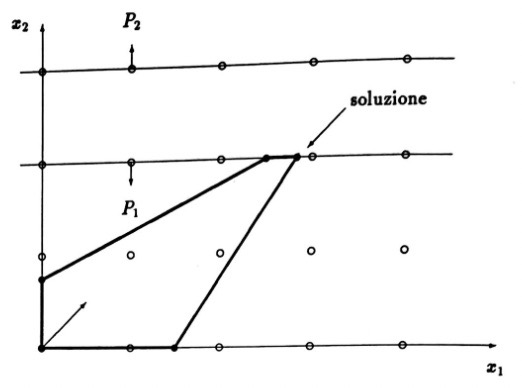
\includegraphics[scale=0.4]{grafbab2.jpeg}
\caption{Regione ammissibile} 
\label{grafbab2}
\end{figure}

dove:

\begin{itemize}
    \item $P_2$ non abbiamo intersezioni quindi è inammissibile
    \item $P_1$ con soluzione ottima in:
        $$x_1 = 2.83,\ x_2 = 2,\ z = 4.83$$
        
        quindi abbiamo upper-bound $4$
\end{itemize}

LA variabile $x_1$ ha valore frazionario compreso tra $2$ e $3$. Effettuiamo un branch con vincoli $x_1 \leq 2$ e $x_1 \geq 3$:

\begin{figure}[H]
\centering
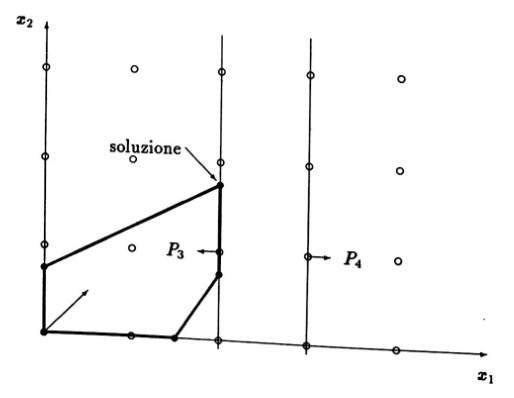
\includegraphics[scale=0.4]{grafbab3.jpeg}
\caption{Regione ammissibile} 
\label{grafbab3}
\end{figure}

dove:

\begin{itemize}
    \item $P_4$ non ha intersezione quindi sarà soluzione inammissibile
    \item $P_3$ con soluzione ottima in:
        $$x_1 = 2,\ x_2 = 1.75,\ z = 3.75$$
        
        quindi abbiamo upper-bound $3$
\end{itemize}

La variabile $x_2$ ha valore frazionario compreso tra $1$ e $2$. Effettuiamo un branch con vincoli $x_2 \leq 1$ e $x_2 \geq 2$:

\begin{figure}[H]
\centering
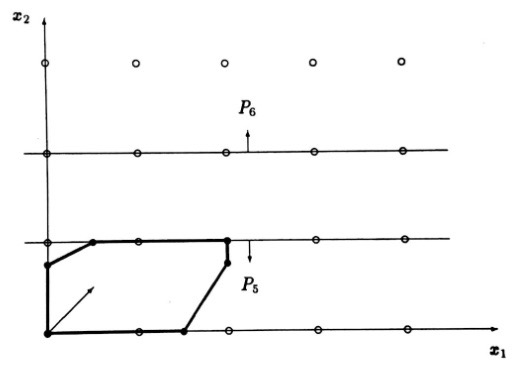
\includegraphics[scale=0.4]{grafbab4.jpeg}
\caption{Regione ammissibile} 
\label{grafbab4}
\end{figure}

dove:

\begin{itemize}
    \item $P_6$ sarà inammissible
    \item $P_5$ con soluzione ottima in:
        $$x_1 = 1, x_2 = 2,\ z = 3$$

\end{itemize}

La soluzione ottima è intera e quindi il branch and bound si interrompe.











nel caso perggiore di variabili binarie il livello computazionele sara dato da O(2^n) quindi il tempo di calcolo cresce esposnenzialmente con il numero di variabili. ma e1 caratteristica di questi problemi  e basta?

se il numero delle varraibili intere n cresce, nel caso perggiore in tempo di calcolo cresce 2^n

in molte applicazionei qundi avremo un tempo di calcolao spaziale di alcune ore o giorni per risolver eil porblema all’ottimo cioe per certificare se un problem non ha soluzioni quidni asssibbile, ci sono sluzioni ammissibili e ela f.o. va da -inf a + inf unbounded o sol ottima. noi vogliamo una soluzione ottima e certificare che avvenga

il porblema e1 il tempo di calcolo ceh ci mette tipo nelgi agenti ceh devono sceglie di fare alcune azioni al posto di altre 
in molte applicazioni si fa affidamente a d algoritimi detti insesatti che CERCANO di generare delle soluzioni ammissibili. ma possono fallire per loro natura

cercano soluzioni ammissibili di buona qualita in un tempo dato 

riesntrano gli algoritmi euristici dove e1 imporporata una conoscenza che ha il progettista e la infonde nell’algoritmo che quindi e1 customizzato 


gli algortimi euristiici sono
- costruttivivi che cercano di generare una priam soluz ammisiibile
- migliorativi che prendo una pirma soluzione e la vcercano di migliiorare e quindi trovare una nuova soluzione con f.o. maggiore se massimizziamo

per alcuni porblemi e§ difficile (time consuming) e quidni ridchied eu ntempo non noto a priori, per questi e1 difficile trvare una soluzoione ottima e risolvere il problema, epr alcuni problemi e1 anche difficile capire se esiste una sluzioe ammissible o no

slide 5


es:
problema del traveling salesman problem
data una matrice C di transizione dve ho che er andare dal punto 1 al 2 pago c_{12} ecc. devo traovare un circuito che tocchi ttutti i punti una sola volta e che abbia costo minimo = somma dei costi di transizione.

tempo di ciclo determina la produttivita della macchina in questo caso immaginiamo un robot che fa n fori e conclusi gli n fori finisce oil cilo

i costi di transizione quindi sono i tempi che il braccio impiega a spostare il braccio da un unto all’altro

troveremo una soluzioneabbissibile tramite unq qualsiasi permutazione in questo caso  ma no  tutte hanno lo stesso costo

le matrici potranno ovviamente essere simmetriche in alcuni casi



cambiando problema prendiamo un veicolo che deve toccare n punti per esempio le consegne di amazon con un solo veicolo e ci potrebbero essere una combinazione come delle finestra temporali di serviziozio dovquindi il veicolo parte da un certo punte a t=0 dal deposito e deve visitare n putnti in finestre temporali prestabiliti come per sempio il punto i nella finestratemporale a_i e b_i
queste finestrre temporali rendono computazionelmente piu difficile o a volte inammissibile il problema

quindi nel caso peggiore il tempo cresce esponenzialmente ad un numero n di cleinti sia pe troavare la solzuione ottima sia per potersi procurare una soluzione ammissiile. la complessita dipende dai dati  e quindi potrebbe esserci una instabilita e uindi cambiando anche solo un datp potremmoavere una soluzioen ammsisibile o una crescita esposnenziale dell’infattiibilita.
 daquesto e1 dovuta l’instabilita


il primo approccio inesatto consiste nell;urae un algorti o branch and bound di tipo troncato

unaltro approccio possibile e1 generare un maniera casuale numeri interi quidni il nostro problema ad n varaibili, generiamo i valori random interi \overline{x}, … ma la soluzione sara ammissibile ma non ottima


approcio di tipo greedy: ingordo

cerca di massimizzare nel breve periodo. procedura sequenzaiale ch costruisce la solzuone un  passo alla volta 
e1 euristica di tipo costruttivo costruiendo la soluzione con un tipo sequenzizale ad ogni passo fa una scelta e massimizza solo l’utilizzo immediato ma cosi puo capirea che
- ho sluzione inammissibile
- non garantisce una soluzione ottima

es: 

pseudocodice greedy o anche detto nearest neighbour: adattamenteo dell’algoritmok greedy al commesso viaggiatore

parto dal punto 1 e lo identifico cole last cioe ultimo punto tocacto 
S={…}e poi una lista di punti da visitare

while non ho toccato tutti i punto S != insieme vuoto
estraggo un punto da S
cerco il punto a costo minimo rispetto al last 
storicizzo il valore del last succesivo
imposto il last alnuovo punto 
end while
riporto il succ last = 1 per poterlo riportare all’inizio


il vantaggio e1 che possiamo prevedere le iterazioni del loop 

es:
n = 4
C = 
0 10 5 8
10 0 2 1 
5 2 0 4
8 1 4 0

last = 1 rho = <2,3,4>
last = 3 ; rho=<2,4>; succ_1 = 3
last = 2; rho=<4>; succ_3 = 2
last = 4; rho =<>; succ_2 =4
succ_4 = 1

ovviamente se abbiamo delle time window l’algoritmo deve essser adattato. quento greedy infati serve per poter essere customizzato per i problemi




classkwork

tramite TSP

usiamo libreira pulp


modello a varaibili binare x_{ij} per ogni coppia di punti i e j ed e1 
- =1 se l’arco x{ij} e1 visistato
- =0 se non e1 viositato

quindi orendiamo le x_{ij} che ci interessano e le imporiamo ad 1 e le altre a 0 dato che queste non fanno parte del nostro “percorso”

img

vogliamo usare la sommatoria {della f.o. }dei costi  dove voglio minimizzarli quindi sostituiamo le x con quelle sopra e le c in base alla tabella dei costi data

secnda somm quindi ogni punto aha un successore
terza sum ogni punto ha un precedessore

quesnti vincoli non basta no per poter risolvere il modello infatti non possiamo esculudere che la soluzione sia disconnessa (sub-tour)


img


dato che mancano dei vincoli di connessione della soluzione


siamo quindi il modello MTZ: miller-zucker0zemlin:
avremo delle variabili addizzionaliu_i una per ogni punto e conu_i rappresenta l’oridine di visitade punto i

imporiamo pertendo dal pnto 1
u_i = 1

abbiamo allora u1 =1 -> x_13 = 1 -> u3 = 2 -> x34 = 1 -> u4 = 3 -> x42 = 1 -> u2 = 4 -> x21 = 1

allora agigungo quenste variabili ui per rappresentare l’ordine di vista e non avere disconitnuita della soluzione

altri vincoli saranno alora:
2 <= ui <= n

dato che le ui con i != 1 saranno comprese tra 2 a n dato che dobbiamo assegnare la 2 posizione finio alla n-esima

poi una ltro vincolo:
ui - uj + 1 <= n(1-xij)

lega le variabili u con xji che dicono cihi viene dopo chi e u l’ordine. questa relaione e1 corretta dato che abbiamo 2 casi:”
- se xij = 0 allora ui - uj +1 <= n ovvio dato che tutte le variabili u son ocomprese in n 
- se xij = 1 allora ui - uj + 1 <= 0 dato che uj >= ui + 1 allora i e1 predecessore di j  alora l;odine di visita di j e1 almeno successivo a i 